\documentclass[endnotes,11pt]{article}
\usepackage{lscape}
%\usepackage{graphics}
\usepackage[pdftex]{graphicx}
\usepackage{color}
%\usepackage{geometry}
\usepackage[margin=1.0in]{geometry}
\usepackage{float}
\usepackage{epstopdf}
\usepackage{mhchem}
\usepackage[small]{caption}
\usepackage{authblk}
%\usepackage{natbib}
%\fontsize{12}{15}
%\geometry{letterpaper,tmargin=1in,bmargin=1in,lmargin=1in,rmargin=1in}
%\setlength{\oddsidemargin}{0cm} \setlength{\evensidemargin}{0cm}
%\setlength{\textwidth}{6.5in} \setlength{\textheight}{9in}


\title{\bf Spectral Library Generating Function for Assessing Spectrum-Spectrum Match Significance }
%\author{Mingxun Wang and Nuno Bandeira}
\author[1,2]{Mingxun Wang}
\author[1,2,3]{Nuno Bandeira}

\date{}

\affil[1]{University of California, San Diego, Dept. of Computer Science and Engineering, 9500 Gilman Dr., La Jolla, CA, 92093, USA \{\texttt{miw023, bandeira}\}\texttt{@ucsd.edu} }
\affil[2]{Center for Computational Mass Spectrometry, CSE, UCSD}
\affil[3]{Skaggs School of Pharmacy and Pharm. Sci., UCSD}

\begin{document}


\maketitle

%\let\oldthefootnote\thefootnote
%\renewcommand{\thefootnote}{\fnsymbol{footnote}}
%\footnotetext[1]{To whom correspondence should be addressed. Email: \url{kinbote@example.com}}
%\let\thefootnote\oldthefootnote

\noindent
{\bf Abstract.}
Tandem mass spectrometry (MS/MS) continues to be the technology of choice for high-throughput analysis of complex proteomics samples. While MS/MS spectra are commonly identified by matching against a database of known protein sequences, the complementary approach of spectral library searching against collections of reference spectra consistently outperforms sequence-based searches by resulting in significantly more identified spectra.
 %(among peptides with spectra in the spectral library).
But while spectral library searches benefit from the advance knowledge of the expected peptide fragmentation patterns recorded in library spectra, estimation of the statistical significance of Spectrum-Spectrum Matches (SSMs) continues to be hindered by difficulties in finding an appropriate definition of `random' SSMs to use as a null model when estimating the significance of true SSMs. We propose to avoid this problem by changing the null hypothesis - instead of determining the probability of observing a high SSM score between randomly matched spectra, we estimate the probability of observing a low SSM score between spectra of the same molecule. To this end, we explicitly model the variation in instrument measurements of MS/MS peak intensities (using a reference spectral library and a set of matching experimental MS/MS spectra) and show how these models can be used to determine a theoretical distribution of SSM scores between reference and query spectra of the same molecule. While the proposed Spectral Library Generating Function (SLGF) approach can be used to calculate theoretical distributions for any additive SSM score (e.g., any dot product), we further show how it can be used to calculate the distribution of expected cosines between reference and query spectra (i.e., under the additional requirement that all query spectra must have Euclidean norm 1). We demonstrate that SLGF-based SSM scores significantly outperform current state-of-the-art spectral library search tools and provide a detailed discussion of the multiple reasons behind the observed differences in the sets of identified MS/MS spectra.
\\
\\
\\
\noindent
{\bf Keywords:} Spectral Libraries, Tandem Mass Spectrometry, Generating Function

\newpage

% \section{Introduction}


High throughput identification of peptides and proteins in complex samples is enabled by tandem mass (MS/MS) spectrometry generation of hundreds of thousands to millions of spectra, from which many thousands of proteins are typically identified by matching the resulting MS/MS spectra against genome-derived databases of known protein sequences~\cite{aebersold03}. In difference from such database search algorithms~\cite{eng94,mascot02,kim10cidetd}, spectral library search approaches~\cite{yates98,stein99,craig06,frewen06,lam07,wang10,yen11,dasari12} identify experimental MS/MS spectra by matching against collections of previously identified reference spectra (spectral libraries) and have been consistently found to identify more spectra than database search whenever the corresponding peptides have reference spectra in the library. But despite this demonstrated superior sensitivity, the development of methods to determine the statistical significance of Spectrum-Spectrum Matches (SSMs) in peptide spectral library searches is still in its early stages.

The most common approach to controlling the False Discovery Rate (FDR) in both database search~\cite{elias07} and spectral library search~\cite{lam10} is the Target-Decoy approach where one extends the database/library of true peptides with a complement of sequences/spectra from `random' peptides and uses matches to the latter to estimate the number of false matches to true sequences/spectra. But while these FDR approaches continue to be very valuable in correcting for multiple hypothesis testing in large-scale experiments, they provide little to no insight on the statistical significance of individual SSMs or Peptide Spectrum Matches (PSMs). In addition, it has been shown~\cite{kim08,kim10cidetd,gupta11} that rigorous modeling of random PSM scores allows one to determine accurate p-values for true PSMs and thus substantially improve the performance of database search tools. In this MS-GF~\cite{kim08} approach, dynamic programming is used to exhaustively determine the distribution of PSM scores for all possible peptides matched to a given spectrum and then this distribution is used to determine the probability (p-value) of observing a random PSM score at least as high as the score of an observed PSM derived from the database of known peptide sequences. Unfortunately this approach does not have a direct analog in the realm of spectral library searches \-- while it is straightforward to traverse the space of all possible random peptide sequences (as in MS-GF), it remains unclear how to generate and/or traverse a space of `random' spectra that would be representative of false matches to a true spectral library.
%
First, truly random spectra~\footnote{For example, all spectra of Euclidean norm 1.0 at a pre-determined fixed resolution for peak intensities.} are easy to generate and could be traversed in a manner similar to MS-GF but such spectra would be mostly very different from the spectra that tend to be generated by mass spectrometry instruments and thus p-values obtained using this background distribution of random spectra would not accurately reflect the probability of false matches for experimental MS/MS spectra.
%
Second, the approach used for the generation of decoy spectra~\cite{lam10} in FDR calculations continues to work well in practice for the generation of small collections of `semi-random' peptide spectra but it is not sufficient to explore the space of {\em all} `random' spectra because it only considers limited changes to peak masses, allows for no variations in peak intensities and is completely peptide-specific in that it is based on sequence permutations (and thus not applicable to spectra from other types of molecules).
%
Third, SSM scoring and p-value approaches have been proposed based on statistical models of random SSMs but these assume uniform distributions of peak masses and either ignore (e.g., hypergeometric models~\cite{yen11,dasari12}) or make limited use (e.g., peak ranks in Kendall-Tau statistic~\cite{dasari12}) of MS/MS peak intensities. As a result, even though these approaches use a probabilistic model and calculate p-values, the underlying assumptions and their results on real MS/MS data suggest that these don't represent the statistics of SSMs well enough to increase the overall number identified SSMs (more details in Results).

%Hypergeometric - easier null model but doesn't take intensity into account and performed significantly worse in the evaluated search results.
%
%Kendall-Tau's incorporation of peak ranks substantially improved the search results but still performed significantly worse than either SpectraST or SLGF.
%
%There has been work using hypergeometric scoring functions that attempt to assess single SSM significance \cite{dasari12, yen11}. However, their null hypothesis, that query spectra are drawn from random spectra, requires modeling of random spectra for use in the calculation of significance. The assumptions made for how these random spectra arise is not completely accurate (i.e. peaks can occur uniformally at random across all m/z values), thus yielding an incorrect null distribution. Additionally, these approaches discard all intensity information from both the library and query spectra. Given the shortcomings of these approaches, the statistics of spectral matching is still an open problem.

%Proteomics is concerned with identifying peptides and proteins in biologically relevant samples. Using high throughput tandem mass spectrometry (MS/MS), yielding MS/MS spectra, combined with computational tools, identification is accomplished. \cite{aebersold03} There are three general approaches to identify these MS/MS spectra are de novo sequencing, database search, and spectral library search. De novo sequencing infers the original peptide sequence only from MS/MS data, thus searching the space of all peptides. Database search utilizes a database of possible peptides derived from predicted gene annotations of a targeted organism's genome. Experimental query spectra are scored against these possible candidate peptides to constitute a peptide spectrum match (PSM).
%%
%Spectral library search is a more sensitive alternative to database search, replacing the database of peptide sequences with a library of identified experimental spectra. \cite{yates98, craig06, frewen06, lam07} Similarly to database search, spectral library search scores matches between experimental query spectra and known library spectra, called a Spectrum-Spectrum Match (SSM). While spectral library searching has been popular in other fields outside of proteomics (e.g. metabolomics \cite{neumann10}), it is with the availability of large curated libraries (e.g. NIST peptide libraries) that has made spectral library searching a viable alternative to database search in proteomics.
%
%In the peptide identification of MS/MS spectra, it is essential to assess the significance of each of these identifications. In de novo sequencing, it is not possible to determine the significance of a peptide identification, as there is no appropriate null distribution for de novo sequencing (Questionable sentence). Database search tools  (e.g. SEQUEST, MASCOT, MS-GFDB, etc.)  \cite{eng94, mascot02, kim10cidetd}, however, are able assess PSM significance. False Discovery Rate (FDR) as calculated using the Target Decoy Method (TDA)  \cite{elias07} is able to calculate the significance of identifications on a set of PSMs and not of a single PSM. MS-GB's generating function approach assesses the significance of a single PSM to a query spectrum. That is, it calculates the probability of a random PSM to a query spectrum with a score exceeding a threshold $T$(by exploring the space all possible peptides), given the null hypothesis that the query spectrum arises from a random peptide. Peptide Spectral Library search, similarly to database, can also utilize TDA \cite{lam10} to determine FDR on a set of query spectra. However, to determine single SSM significance, state of the art search tools (e.g. SpectraST \cite{lam07}) utilize scoring functions that lack the ability to assess significance of SSMs. If one were to use a similar null hypothesis as MS-GF (i.e. query spectra arise from a random peptide), it would be possible to calculate null distribution by iterating over the space of all peptides and calculating the distribution of scores between the query and the spectra that would arise from these peptides (using tools as Mass Analyzer \cite{zhang04}). Yet, exploring such a large search space is infeasible through explicit enumeration.
%
%There has been work using hypergeometric scoring functions that attempt to assess single SSM significance \cite{dasari12, yen11}. However, their null hypothesis, that query spectra are drawn from random spectra, requires modeling of random spectra for use in the calculation of significance. The assumptions made for how these random spectra arise is not completely accurate (i.e. peaks can occur uniformally at random across all m/z values), thus yielding an incorrect null distribution. Additionally, these approaches discard all intensity information from both the library and query spectra. Given the shortcomings of these approaches, the statistics of spectral matching is still an open problem.
%
%Given the difficulty of modeling random spectra or efficiently modeling spectra from the entire space of all random peptides (or compounds), we propose using a different null hypothesis to assess the quality of SSMs. Instead of determining the probability of a random match with a score $\ge T$, we propose to determine the probability that a \emph{true} match has a score $\le T$. Intuitively, this can be determined for a given compound by using a reference spectrum of that compound and knowledge of the expected variation caused by instrument measurement error \cite{tabb10, venable04}. In our approach called Spectral Library Generating Function (SLGF), we modeled how peaks in a library spectrum can change in replicate spectra and we calculated how these changes ultimately affected similarity scores in order to assess the significance of single SSMs.

Given the difficulty of modeling random spectra, we propose changing the null hypothesis used to assess the significance of SSMs \--- instead of determining the probability of a random match with a score $\ge T$, our approach determines the probability that a \emph{true} match has a score $\le T$. While modeling true matches remains a open problem in database search due to the difficulty of predicting theoretical MS/MS spectra from peptide sequences, we show that these can be efficiently modeled in the case of spectral library searches using $i$) advance knowledge of expected fragmentation patterns as recorded in reference library spectra and $ii$) estimated models of instrument variation in measurements of MS/MS peak intensities. Our Spectral Library Generating Function (SLGF) approach combines these with an efficient dynamic programming exploration of all possible {\em replicate} spectra of the same molecules as each reference spectrum in the library to output a spectrum-specific theoretical distribution of scores for true SSMs.
%
In addition to defining a new approach for the assessment of the statistical significance of SSMs, our comparison of SLGF with current state-of-the-art spectral library search tools shows that SLGF significantly increases the number of identified MS/MS spectra without requiring any peptide-specific assumptions or multi-feature corrections to observed cosine scores (e.g., DeltaD/DotBias).

%Intuitively, this can be determined for a given compound by using a reference spectrum of that compound and knowledge of the expected variation caused by instrument measurement error \cite{tabb10, venable04}. In our approach called Spectral Library Generating Function (SLGF), we modeled how peaks in a library spectrum can change in replicate spectra and we calculated how these changes ultimately affected similarity scores in order to assess the significance of single SSMs.

%Spectral library searching has recently gained traction as a via tool to identify compounds, biologically significant molecules, in high throughput mass spectrometry experiments. These mass spectrometry experiments attempt to identify compounds within a biological sample using liquid chromatography to chromatographically separate different compounds. Ionization of these compounds yields precursors (a compound with a unique charge) which are subsequently selected based upon their mass to charge (m/z) ratios. These precursors are broken down into smaller fragments (using Collision Induced Disassociation(CID) for example) \cite{domon06} to be measured by a mass spectrometer yielding a spectrum ( (mass, intensity) pairs) in a process called tandem mass spectrometry (MS/MS).

%In proteomics, tandem mass spectrometry is used extensively to assay proteomic samples. To identify these proteomics MS/MS spectra, traditionally database search tools \cite{aebersold03} (e.g. SEQUEST, MASCOT, MS-GFDB, etc.) \cite{eng94, mascot02, kim10cidetd} take on the task, matching and scoring these spectra to a possible peptide sequences in a Target database of proteins derived from genes in annotated genomes. In these database search tools, the False Discovery Rate (FDR) is estimated using the Target Decoy Approach (TDA) \cite{elias07}. Briefly, TDA generates a Decoy database from the Target database by simply reversing all amino acid sequences. This Decoy represents a random set of peptide sequences that is assumed to correctly model the likelihood of the MS/MS spectra to match randomly to the Target database thus giving us an estimate of the FDR.

%These database tools' shortcomings are their inability to accurately, either explicitly or implicitly, model peptide fragmentation. Spectral Library search offers an alternative by replacing database peptides strings with previously identified experimental spectra \cite{yates98, craig06, frewen06, lam07}. Instead of matching these unknown MS/MS spectra (known as Query spectra) against peptide sequence in a protein database, these query spectra are scored matched against known spectra in a spectral library (known as Library spectra). This pairing scoring of Query and Library spectrum is known as a Spectrum-Spectrum Match (SSM).

%While spectral library searching has increased sensitivity in identifying spectra from MS/MS experiments, current spectral library search is limited in that many of state of the art library search tools use scoring schemes which have no meaning of significance for single spectrum-spectrum matches. Instead, these approaches rely upon false discovery rate (FDR) estimated by the TDA of a set of spectra to roughly estimate significance \cite{lam10}. It is preferable to have a theoretical statistical significance for these spectrum-spectrum matches. There have been some attempts to use hyper-geometric scoring functions to assess significance, but these approaches discard much of the intensity information of the MS/MS spectra. \cite{yen11, tabb12},

%MS-GF \cite{kim08}, an approach from Proteomic database sequence searching, uses generating functions that yield rigorous p-values for database search given the null hypothesis that a query spectrum is derived from a random peptide in the space of all possible peptides. MS-GF is able to compute statistical significance of single peptide spectrum matches by calculating the probability of a random match exceeding a peptide spectrum match (PSM) score.  To maintain the same null hypothesis for SSMs would involve modeling spectra of random peptides using a method similar to SpectraST's shuffle and reposition decoy creation approach which is unsuitable for dynamic programming algorithms. This would be more similar to X!Tandem's E-value \cite{fenyo03} estimation rather than MSGF's rigorous p-values.

%Given the futility of modeling random spectra or efficiently modeling spectra from the entire space of all random peptides, we propose a change of the null hypothesis. We can now presume that a query peptide is a replicate of a library spectrum instead of a random spectrum in our null hypothesis. We attempt to model how peaks in a library spectrum can change in replicate spectrum and how they can ultimately affect spectral dot product scores. Ion intensity variation, ion deletion, and ion insertion (caused by noise or co-elution) are all factors that can severely affect SSM similarity. In our approach called Spectral Library Generating Function (SLGF), we aim to model intensity variation and ion deletion and to calculate the significance of single SSMs.


\subsection*{Methods}

%\subsection{Spectrum Spectrum Match similarity}
A spectrum is defined as a set of (mass, intensity) pairs called peaks which are assigned into uniformly sized mass bins (e.g. 1 Th bins \cite{frewen06}). After transformation~\footnote{We note that even though spectrum binning is used here for ease of explanation of our approach, the actual implementation uses peak lists to improve performance as well as to provide the ability to use per-peak m/z tolerances.} a spectrum becomes a vector $S$ with $n$ bins, where each bin $S_i$ contains the summed intensity of all peaks with masses in that bin; all subsequent references to ``spectrum'' refer to the respective spectrum's vector. Given a library spectrum $L$ and a query spectrum $S$, the projection spectrum $Proj(S,L)$ is defined as:
$$
Proj(S,L) = \{{S_i : (L_i > 0), 0 \ otherwise\}}
$$
All library spectra $L$ are normalized to euclidean norm $||L|| = 1.0$, as are all projected spectra:

%A normalized projected query spectrum is a projected query spectrum that has its bins intensities normalized by the euclidean norm.

$$
S^L = NormProj(S,L) = \left\{ \frac{Proj(S,L)_i} {||Proj(S,L)||} \right\}, \ where \ ||Proj(S,L)|| = \sqrt {\sum_{i}{Proj(S,L)_i^2 } }
$$

The most common spectral similarity function used for spectral matching is cosine (also known as normalized dot product), defined as follows for vectors of Euclidian norm 1.0:

$$
cos(L,S^L) = \sum_{i}{L_i \times S^L_i}
$$

%\subsection{Ion Variance Model}
We define a replicate spectrum $R$ (relative to a library spectrum $L$) to be a spectrum of the same molecule as $L$ and acquired under the same or similar  experimental conditions (i.e., charge state, instrument, collision energy, abundance, etc.). Due to stochastic factors in mass spectrometry fragmentation and instrument measurement error \cite{venable04}, some level of variation is expected between the intensities of peaks in $R$ relative to the intensities of peaks in $L$. We model this variability with a log ratio of ion intensities, $log ( R^L_i / L_i )$ where $R^L = NormProj(R,L)$; this ratio is calculated across all bins in $R$ and $L$ where $L_i$ is not zero.

For all library spectra with replicate spectra in our training datasets, all observed log ratios were collected into an ion variation histogram. We use this histogram (scaled to total area under the curve 1.0) as the empirical probability mass function, $RatioFreq(r)$, of variation in ion intensities for all $L_i \neq 0$ (Figure~\ref{Paths}A). In difference from varying intensities, the special cases of ion deletion (i.e., $R_i^L = 0$) are modeled separately with $DelFreq = \frac{\#Deletions}{\#Replicates \times \#Peaks\_in\_library\_spectrum}$, where $\#Deletions$ is the total number of peak deletions in replicate spectra, $\#Replicates$ is the total number of replicate spectra in our training set, and $\#Peaks\_in\_library\_spectrum$ is the total number of peaks in all library spectra. Combining our model of ion variance, $RatioFreq(r)$, and our model for ion deletion events $DelFreq$, the probability $Prob( R_i | L_i)$ of observing a replicate ion intensity $R_i$ given a library ion intensity $L_i$ is:

$$
Prob( R_i | L_i) =
        \left\{ \begin{array}{ll}
            DelFreq & \mbox{if\ } R_i = 0\\
            (1-DelFreq)\times RatioFreq( \log_2( \frac{ R_i }{ L_i }  )) & \mbox{if\ } R_i\neq 0
        \end{array}
        \right.
$$




%\subsection{Generating Function}
Our goal is to calculate the distribution of cosines scores over all possible replicate spectra within instrument variability of a given library spectrum. To compute the generating function for each library spectrum, we use $RatioFreq$ and $DelFreq$. We consider every possible replicate spectrum $R$ (Figure~\ref{Paths}B) by exploring all possible intensity variations of every peak $L_i$ to $R_i$ and calculate their aggregate probability and cosine similarity $cos(R^L, L)$.

\begin{figure}[h!]
 \centering
	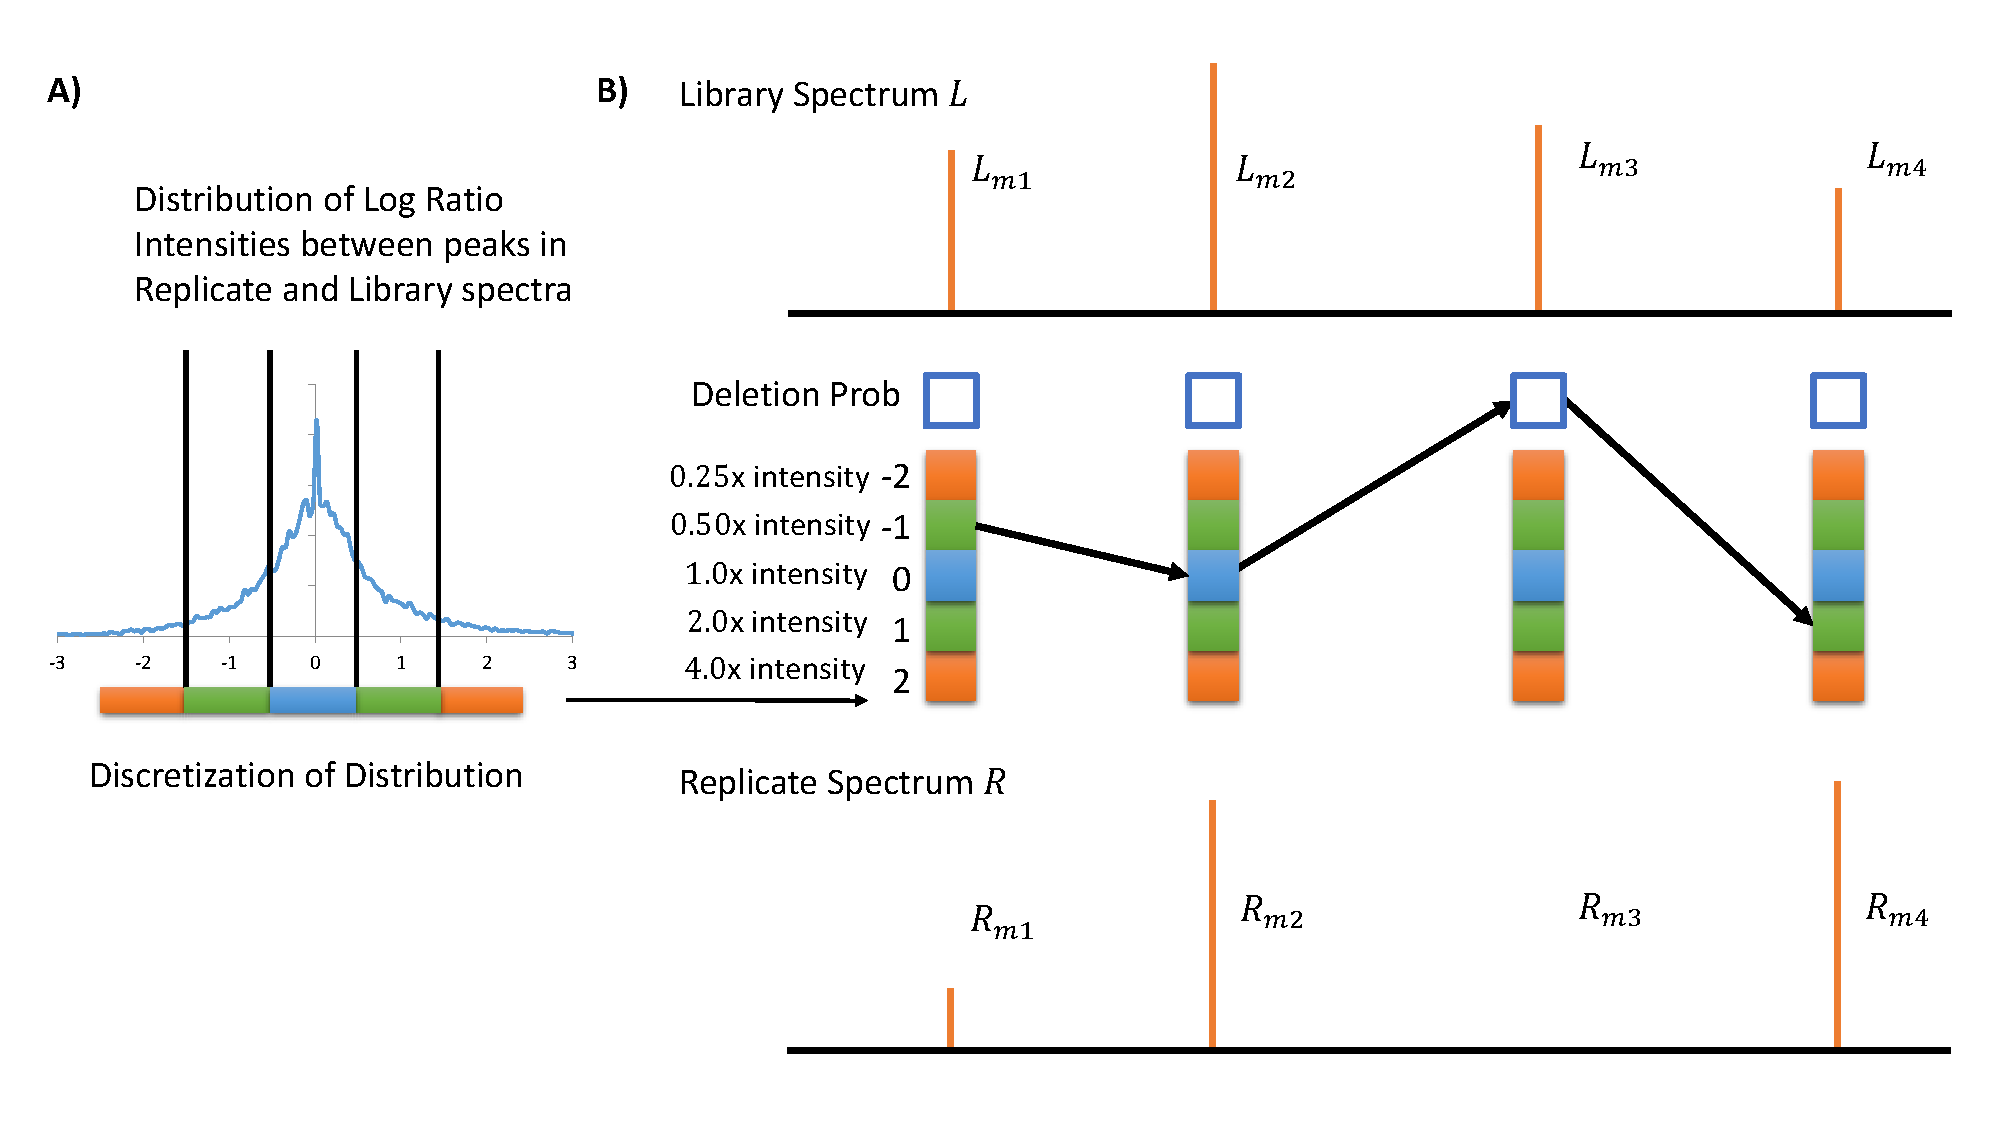
\includegraphics[scale=0.50]{SLGFPaths2.pdf}
	\vspace{-0.30in}
  \caption{Spectral Library Generating Function (SLGF) calculation of Spectrum-Spectrum Match (SSM) significance by modeling instrument variation in peak intensity measurements in replicate spectra of the same compound. In (A) the empirical distribution of variations in intensity measurements is assessed and discretized. (B) Every possible replicate spectrum $R$ is represented by a path through each library peak's possible intensity variations, thus representing every possible combination of variations of peaks in library spectrum $L$. Note that some replicate spectra (paths) are invalid, i.e. replicate spectra that do not have Euclidean norm 1; intermediate paths with norm $<1.0$ are allowed during the calculation but paths resulting in norm $>1.0$ must be discarded when calculating the distribution of cosine scores. }
	\label{Paths}
\end{figure}


A three dimensional dynamic programming table, $LibDP(i,c,p)$, is used to explore all possible ion variations, where $i$ is the spectrum vector index, $c$ is the cosine score, and $p$ is the summed squared intensity used. The value in each cell $LibDP(i,c,p)$ is the probability of a replicate spectrum obtaining cosine $c$, using $p$ squared intensity, and up to and including ion index $i$.
The recurrence for $libDP(i,c,p)$ is thus defined as follows for $i=1..n$:
$$
LibDP(i,c,p) = \sum_{y=0\rightarrow p}
   LibDP( i-1, c-\sqrt{y}\times L_i, p-y ) \times Prob( \sqrt{y} | L_i)
$$
At ($i=0$), before considering any ions from the library spectrum $L$, every cell $LibDP(0, >0, >0) = 0$, and when no intensity is used and the cosine score is zero, it is $LibDP(0,0,0) = 1$.

Since each step $i$ only depends on the values from step $i-1$, one only needs to use two two-dimensional matrices of constant size to calculate all $LibDP$ values. The size of each 2D matrix is $n_c \times n_p$, where $n_c$ is the number of cosine bins and $n_p$ is the number of intensity bins, each set accordingly to the desired granularity. The time complexity of complexity of computing the entire dynamic programming table is $O(n_c \times n_p^2 \times n)$. The final SLGF distribution of cosines between a library spectrum and its replicates is extracted from $LibDP(n, *, 1)$ and normalized to sum to 1. It is necessary to normalize at the end because of probability mass in discarded replicate spectra of Euclidean norm $\neq 1$.

%\subsection{SSM significance calculation}
The probability that a replicate spectrum $R$ and corresponding library spectrum $L$ exhibit a cosine less than a threshold is expressed as the following p-value:
$$
Prob_L ( cos(L, R^L) < T  )
$$
where $T$ can be set according to observed cosines between query and library spectra to determine the probability of a query spectrum $S$ being a replicate spectrum of $L$.


%\subsection{SLGF as a score}
SLGF assesses the quality of a single SSM but does not correct for multiple hypothesis testing when searching many spectra in a dataset. To address this for peptide spectral libraries, we used the FDR calculation estimated by the TDA~\cite{lam10}. In brief, Decoy spectral libraries were generated using the peptide shuffle and reposition method to obtain a set of decoy spectra. For all Target and Decoy library spectra, SLGF distributions were calculated and used in the subsequent scoring function.


The scoring function of an SSM in the spectral library search between a library spectrum $L$ identified as $Peptide(L)$ and a query $S$ is:
%$$
%SSM_{score} = SLGF_e = SLGF_{pvalue}(cos (L, S^L), L) \times
%			Explained Intensity (S, Peptide(L))
%$$
$$
SSM_{score} = SLGF_e = Prob_L ( cos(L, R^L) < cos (L, S^L)  ) \times
			Explained Intensity (S, Peptide(L))
$$

The score $SLGF_e$ is also considered in addition to
% $SLGF = SLGF_{pvalue}(cos (L, S^L), Library)$
$SLGF = Prob_L ( cos(L, R^L) < cos (L, S^L)  )$
because it is a closer comparison to SpectraST~\cite{lam07}, which does not consider co-eluting peptides. In cases of co-eluting peptides, $SLGF$ is able to consider these spectra because it only uses peaks at m/z values $L_i\neq 0$. Yet since SpectraST penalizes for co-elution, $SLGF_e$ is similarity penalized by the explained intensity term. While SLGF may be useful towards identification of co-eluting peptides, additional considerations are required to correctly address co-eluting peptide identification~\cite{wang10} (e.g., addressing multiple molecules per spectrum and FDR on mixture identifications).

\subsection*{Datasets}

%subsection{Datasets}
The {\em Training dataset} was composed of 236 CPTAC~\cite{paulovich10,tabb10} Study 6 Orbitrap files (2,766,504 spectra) and was used to train the distributions of variation in ion intensities. All spectra were searched with SpectraST v4.0 with a 2 Th m/z tolerance against the NIST Yeast Ion Trap peptide library (May 2011 build). The decoy spectral library was created using SpectraST's own decoy generation feature and the resulting SSMs were filtered to 1\% FDR, yielding 396,526 identified spectra from 18,440 unique precursors. Replicate spectra in this filtered dataset were matched with their respective library spectra in the library and ion variance distributions were calculated from these replicates and library spectra.

The {\em Test dataset} from CPTAC was composed of an arbitrarily selected file from CPTAC Study 6 that was \emph{not} included in the Training dataset and contained 9,809 MS/MS spectra used for evaluating SLGF's search of the NIST Yeast Ion Trap peptide library (May 2011 build). The shuffle and reposition method proposed by Lam~et~al~\cite{lam10} was used to create the decoy spectral libraries for use in both SLGF's search as well as SpectraST's and Pepitome's search. SpectraST, Pepitome, and SLGF searched the NIST library using a 2 Th precursor tolerance; SLGF and Pepitome used a 0.5 Th tolerance to annotate MS/MS peaks.

A second test dataset, {\em Hela S3 Test} dataset, was also used to evaluate spectral search performance in addition to the CPTAC {\em Test dataset} described above. This dataset, described previously in ~\cite{rudomin09}, is from human HeLa S3 cells. The sample was tryptically digested, chromatographically separated over 90 minutes, and analyzed by an LTQ Orbitrap Classic. {\em Hela S3 Test} contained 11723 MS/MS spectra and was searched against the NIST Human Ion Trap peptide library (May 2011 build). 

For SLGF peptide spectra library search we find that it is best to perform library preprocessing. Peaks in library spectra were annotated with the respective peptide sequence considering $b$,$y$,$b$++,$y$++ ions~\cite{Roepstorff84}, their respective single $^{13}C$ isotope peaks ($+1$ Da mass shift), single \ce{H_{2}O} losses ($-18$ Da mass shift), single \ce{NH_{3}} ($-17$ Da mass shift) losses and $a$ ions; all non-annotated peaks and precursor peaks were removed. Additionally, all peak intensities were transformed by square root in both library and query spectra.

\subsection*{Results and Discussion}

In calculating the SLGF distributions for each peptide library spectrum, it was observed that it was more accurate to have 10 different distributions of variation in ion intensity based on the relative abundance of an ion peak in the library spectrum (instead of a single distribution for all ion peaks). Figure~\ref{IonVariances} illustrates the significant differences in the distributions of log-ratio ion variations for the top 10\% most intense peaks and bottom 10\% least intense ion peaks (other deciles also shown). Additionally, the ion variance is also substantially different between replicate spectra from high ($\geq 12,000 $ ions) and low abundance ($<12,000 $ ions) precursors. The abundance of a spectrum is calculated as the total ion current of that MS/MS spectrum. As expected, low intensity replicates exhibit more variation in ion intensities (i.e., wider ion variation distributions) than high intensity replicates. Using these two separate models for high and low abundance precursors, two SLGF distributions are pre-calculated for each library spectrum. Low and high abundance query spectra are then partitioned and searched separately, with SLGF p-values calculated from the corresponding SLGF distribution.

\begin{figure}[h!]
 \centering
	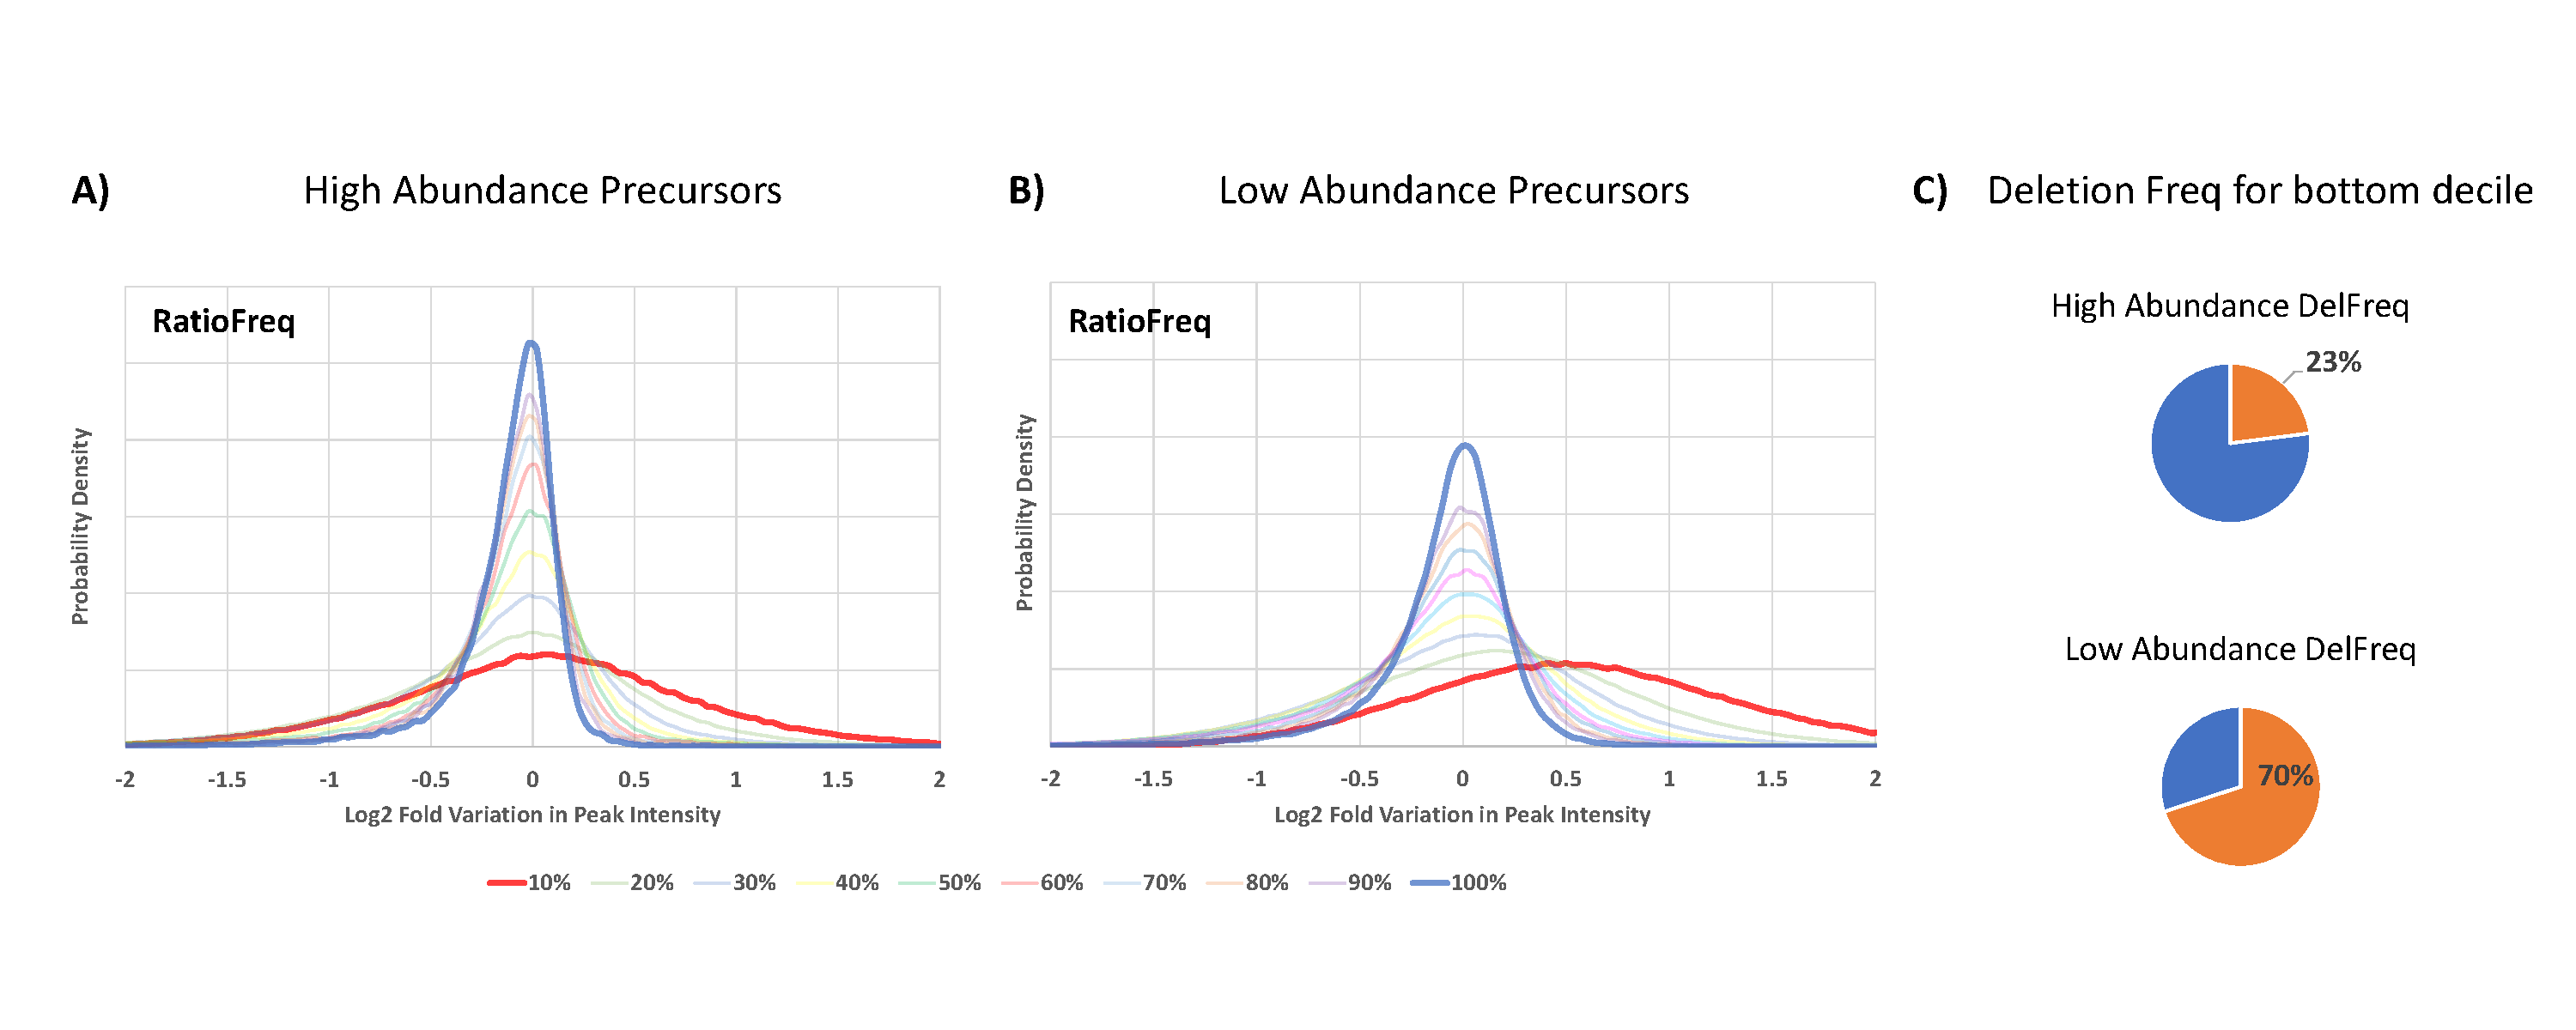
\includegraphics[scale=0.33]{IonVariances4.pdf}
	\vspace{-0.5in}
  \caption{Distributions of variation in ion intensity for (A) high and (B) low abundance precursors. As illustrated by the differences between (A) and (B), the ion variation distributions for low abundance precursors tend to be wider than those of the high abundance precursors. In both cases it is shown in bold blue, the distribution of variation in ion intensities for the 10\% most intense peaks in library spectra and in bold red, the distribution of variation in ion intensities for the 10\% least intense peaks in library spectra, with other deciles shown in between. Note that the width of the distributions for the top decile distribution is markedly narrower than the bottom decile distribution suggesting the need to model the variation of ion intensity differently depending upon a peak's intensity in the library spectrum. It should also be noted that the lowest decile distribution shown in (B) in red is not centered at 0 log fold variation due to the significantly higher deletion percentage (C) of the lowest decile library peaks in low abundance precursors. The deletion of these peaks caused all other peaks in the spectrum to increase in normalized intensity, for the entire spectrum is normalized to Euclidean Norm 1, thus causing a shift in the specific ion variation distribution. }
	\label{IonVariances}
\end{figure}

The SLGF distributions were visually assessed by comparing against empirical score distributions using replicates from the Training dataset, and it was found that SLGF distributions approximated the empirical distributions (See Figure~\ref{SLGFvsEmpirical}), but further work is necessary to enable a more accurate p-value calculation. Thus, we use SLGF p-value as a score and evaluate its performance in the context of spectral library search.



\begin{figure}[!h]
 \centering
	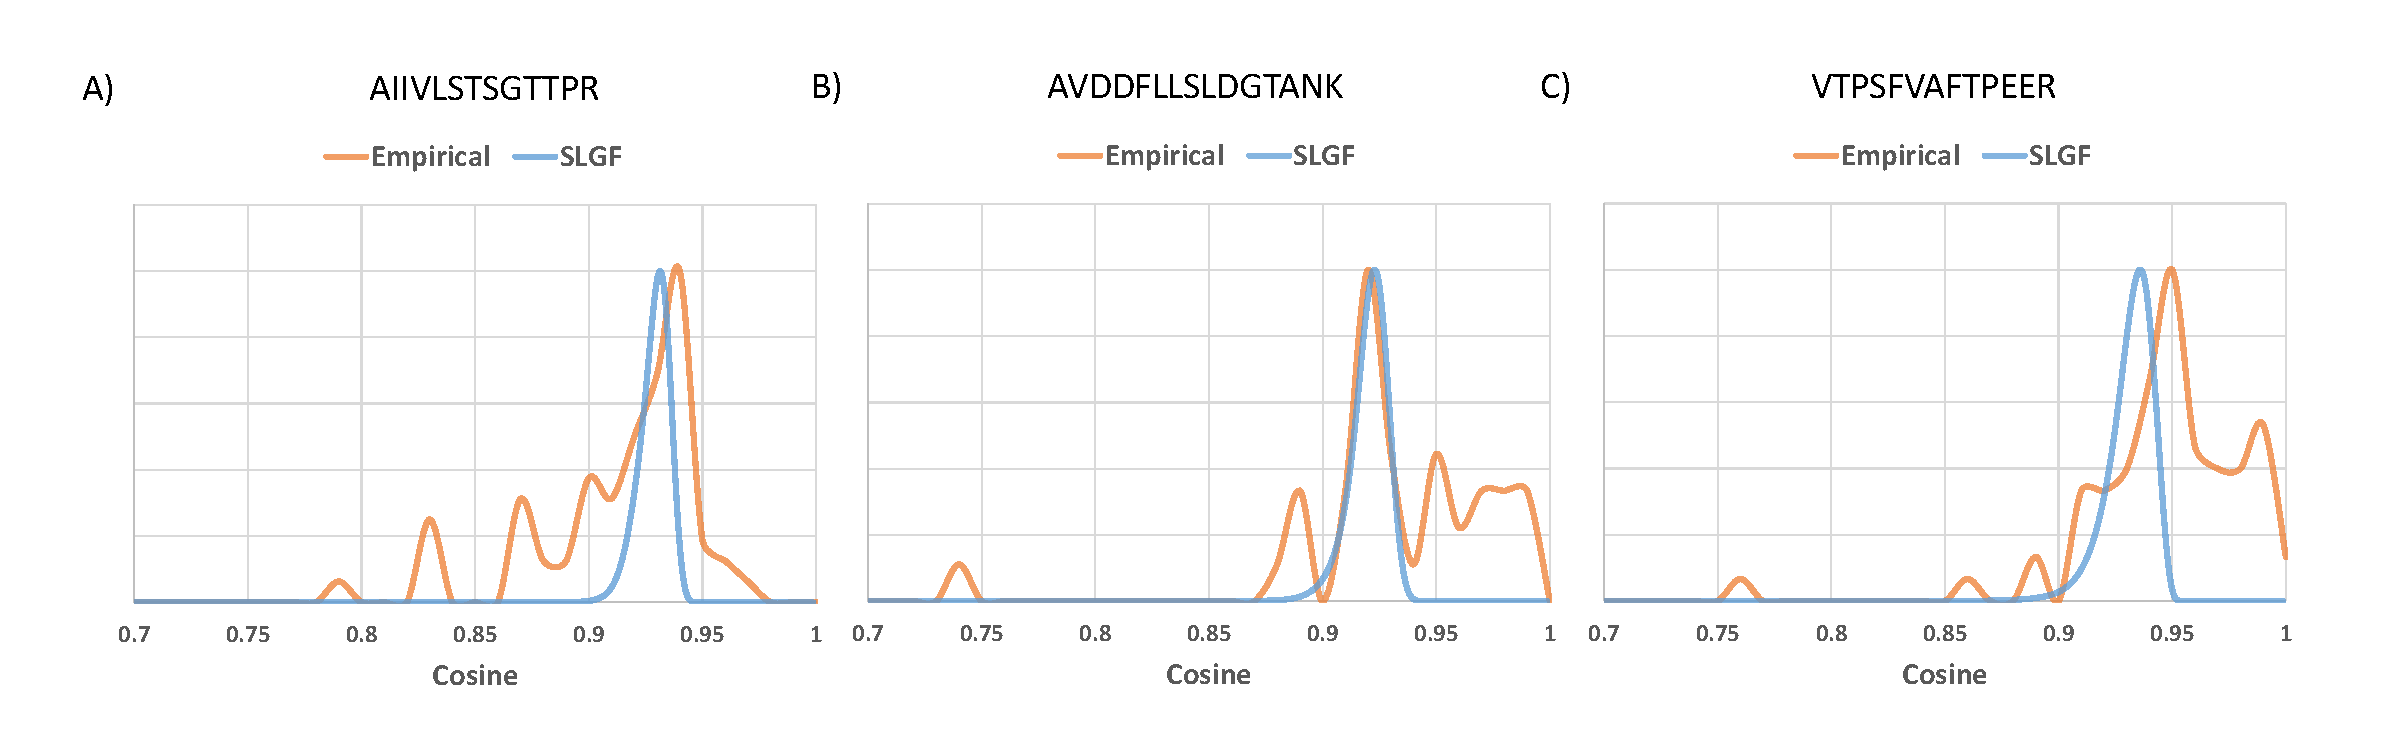
\includegraphics[scale=0.42]{SLGFEmpiricals2.pdf}
	\vspace{-0.3in}
  \caption{Empirical vs calculated (SLGF) distributions of cosines between library and replicate spectra. Examples were selected from library spectra with sufficient replicates to derive an empirical distribution. The probability mass in the empirical distributions to the left of the theoretical SLGF distribution is mostly caused by cases of co-elution, leading to lower cosines. The discrepancies of higher cosines result from SLGF using an average model of ion variation derived from data acquired in many experiments and laboratories. As such, our average model of ion intensity variation for certain peptides has variance higher than that of the best calibrated instruments, thus causing SLGF distributions to expect lower average cosines than some empirical distributions. }
	\label{SLGFvsEmpirical}
\end{figure}


\subsubsection{Peptide Spectral Library Search}


To systematically assess the performance of SLGF as a search tool, we compared it against SpectraST and Pepitome at fixed FDR. Given that the performance of SpectraST substantially exceeded that of Pepitome, we focus our detailed analysis on the comparison with SpectraST results. Comparing the sensitivity of SLGF to that of SpectraST on the Test dataset we find that at 1\% spectrum-level FDR (as determined by TDA), SLGF was able to identify 4,373 spectra versus 3,884 spectra by SpectraST (12.5\% more, see Figure~\ref{SLGFSearchROCVenn}).

\begin{figure}[!h]
 \centering
	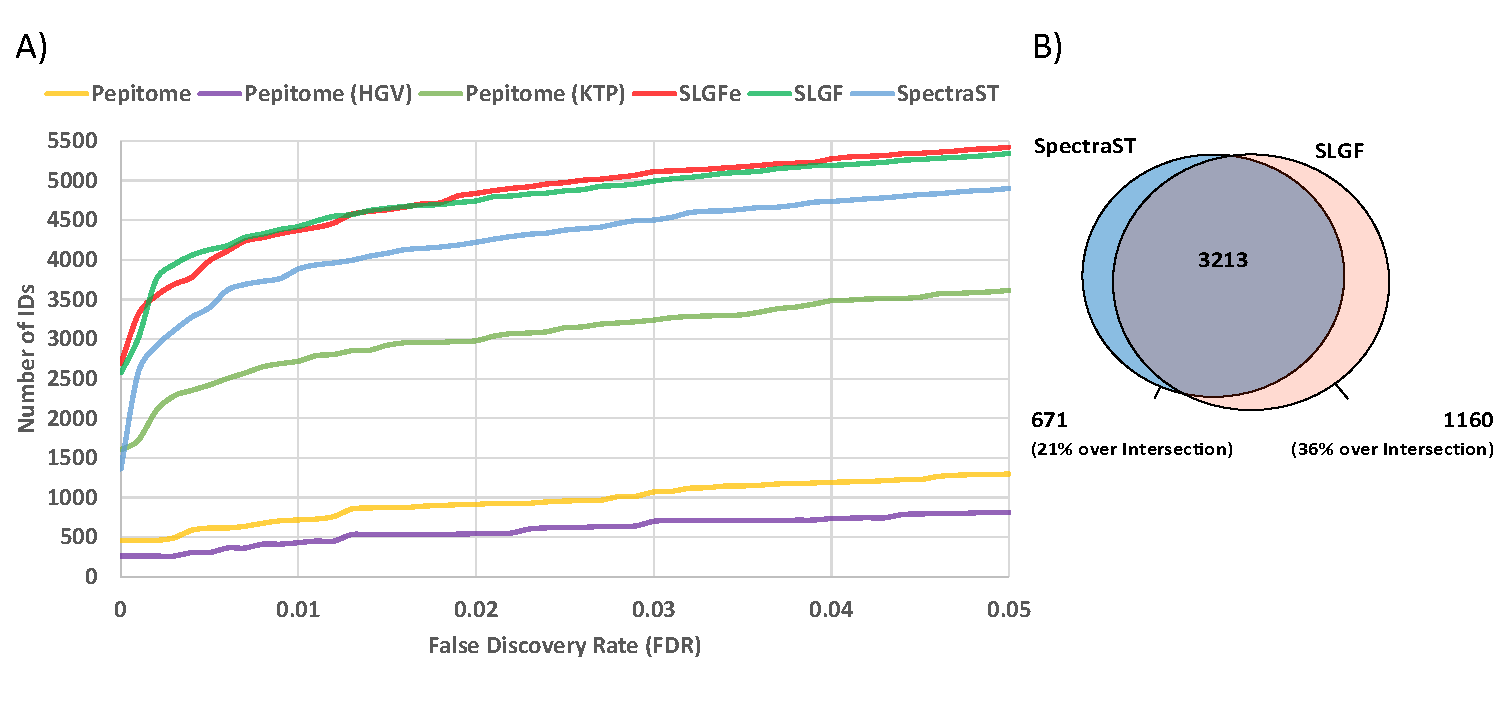
\includegraphics[scale=.64]{ROCCurve_Venn5.pdf}
	\vspace{-0.2in}
  \caption{Peptide spectral library search sensitivity and specificity comparison between SLGF, SpectraST, and Pepitome.  In (A) the performance of the scoring function $SLGF$ is shown to be comparable to that of $SLGF_e$, where one explicitly attempts to not consider mixture spectra (see text for details). This contrasts to the performance of SpectraST in blue and Pepitome in yellow. Note that alternative rankings of Pepitome's search results based upon Pepitome's hypergeometric score (HGV) and Kendall-Tau p-value (KTP) perform worse and and better, respectively, than Pepitome's default combination of several scores (B) Number of spectra identified exclusively by SpectraST, SLGF, and by both tools at 1\% spectrum level FDR. On this Test dataset, SLGF was also found to be more sensitive than SpectraST across the whole range of FDR thresholds ($>12\%$ increase in IDs at 1\% FDR)}
	\label{SLGFSearchROCVenn}
\end{figure}

% As seen in Figure~\ref{SLGFSearchROCVenn}B , 3213 spectra were identified by both SpectraST and SLGF. 1160 spectra were only identified by SLGF and 671 spectra were only identified by SpectraST at 1\% FDR.

 The gain in SLGF sensitivity can be explained by analyzing the different components in SpectraST's SSM scores. SpectraST's score is $SSM_{spectrast score} = 0.6D + 0.4DeltaD - b$, where $D$ is the cosine score between library and query. $DeltaD = \frac{D_1 - D_2}{D_1}$ where $D_1$ and $D_2$ are the top and second cosine scores respectively from a set of library spectra to a query spectrum. It is argued that the larger this $DeltaD$ term, the more the top candidate stands out from the alternatives, thus implying a greater chance the top candidate is correct. $b$ is the penalty applied to the score for $DotBias$ scores that are not preferable. $DotBias$ is defined as $DotBias = \frac{\sqrt{\sum_{i=1 \rightarrow n}{L_i^2 * (S^L_i)^2} }} {D}$ and intuitively can be thought of a measure of how much a cosine score is dominated by a few peaks. A score of $DotBias=1.0$ signifies one peak dominates the score and a score of $DotBias\approx0.0$, the cosine contribution is evenly distributed over all peaks. Thus, high $DotBias$ scores possibly imply dubious matches as there are only a few peaks leading to a high cosine score. Low $DotBias$ scores also are not preferable as this means many equal intensity peaks are matching, which most likely would imply noise. SpectraST's penalty $b$ is tuned to cause larger penalties for larger and very small $DotBias$ values. In figure~\ref{SLGFDeltaDotBias}A it is shown the $DeltaD$ versus the $DotBias$ of all IDs at 1\% FDR identified by SpectraST over the test dataset (orange dots). As expected SpectraST IDs tend to avoid high $DotBias$ as well as exceedingly low $DeltaD$. In difference from these, SLGF-only IDs are shown in gray dots. These tended towards lower $DeltaD$ and higher $DotBias$ and thus were missed by SpectraST, because of either low $DeltaD$ (lacking the ability to distinguish between the top two SSMs) or because of high $DotBias$ (cosine score dominated by only a few peaks). SLGF, however, is able to identify these low $DeltaD$ spectra because each possible library match to the query spectrum has a different expected score distribution, and even though from an absolute cosine perspective there is little difference from the top and second hit, once the cosine p-value is calculated for each respective library spectrum, then the scores separate substantially. It is clearly show in figure~\ref{SLGFDeltaDotBias}B that even though the $DeltaD$ for these spectra that SpectraST failed to identify was very low (x-axis), the SLGF's delta score ($SLGF_{delta} = \frac{SLGF_1 - SLGF_2}{SLGF_1}$ where $SLGF_1$ and $SLGF_2$ are the top and second SLGF scores respectively) is considerably higher because of the separation obtained from SLGF p-values.

The identification of spectra with high $DotBias$ is also enabled by the calculated cosine distribution. For spectra whose intensities are dominated by very few peaks, cosines alone are not enough to distinguish between good SSMs and bad SSMs. Since these spectra are dominated by few peaks, the less intense peaks become especially informative in how their slight cosine changes (because of matching or not matching these small peaks) distinguish good and bad SSMs. SLGF's distributions are able to capture these slight changes in cosine (i.e. higher SLGF distributions with lower variance) to correctly identify spectra dominated by few peaks whereas SpectraST penalizes \emph{all} spectra that are dominated by a few peaks. In general we observe that the effect of $DeltaD$ is captured by SLGF's determination of the appropriate mean cosine per library spectrum and the effect of $DotBias$ is captured by the variance of the SLGF distributions.

An additional source of IDs that SLGF was able to recover were spectra that SpectraST did not consider in its search: spectra that have ``negligible'' abundance above 500 m/z. These spectra generally came from shorter (6-8mer) charge 2 precursors and moderate length (8-12mer) charge 3 precursors. While these spectra may be easier to match to decoys with SpectraST's scoring scheme, SLGF is again able to use its calculated distributions to identify 198 spectra that SpectraST discarded.


\begin{figure}[!h]
 \centering
	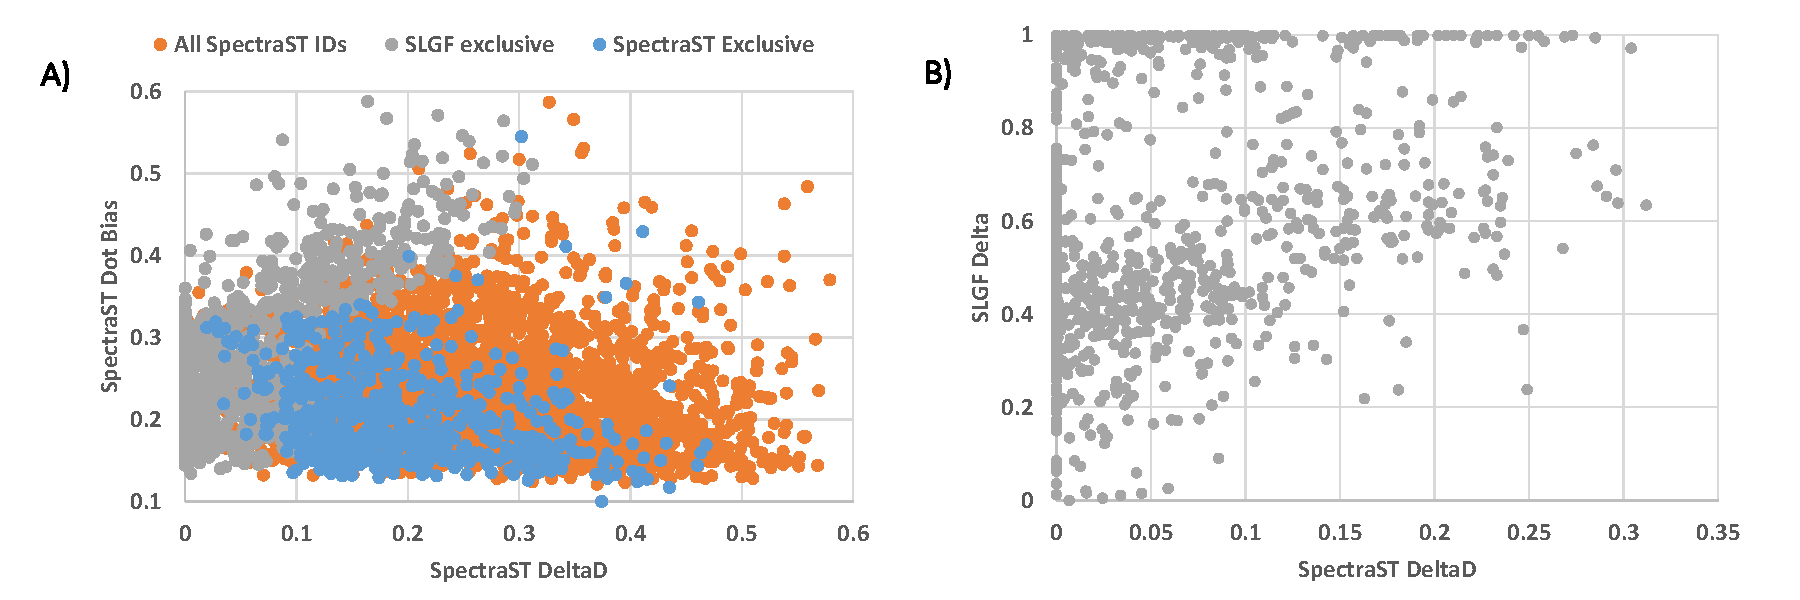
\includegraphics[scale=.55]{DotBiasVsDeltaD2.pdf}
	\vspace{-0.3in}
  \caption{ Gains of identification by SLGF over SpectraST through analyzing SpectraST's score's $DotBias$ and $DeltaD$. Each dot in (A) represents an identified spectra plotted with DeltaD versus $DotBias$ as calculated by SpectraST. In orange are all the IDs by SpectraST; in blue are the identifications by SpectraST at 1\% FDR that were missed by SLGF's search at 1\% FDR; in gray are the identifications by SLGF at 1\% FDR that were missed by SpectraST at 1\% FDR. For this third category of spectra, there is a clear bias towards high $DotBias$ and low $DeltaD$. It is shown in (B) that while SpectraST was unable to obtain a large DeltaD for these spectra, SLGF's delta score was high and, since this delta score is not used anywhere in SLGF scores, it thus reinforces the assertion that these SLGF identifications are correct. SLGF's exclusive identifications show that there are classes of spectra that remained unidentified (low $DeltaD$ and high $DotBias$) that SLGF is now able to identify. Note the change of scale for the DeltaD axis (x-axis) in B as opposed to A; since there were no spectra with SpectraST DeltaD $>0.35$ we opted to omit those regions in the figure. }
	\label{SLGFDeltaDotBias}
\end{figure}


The 671 spectra that were identified by SpectraST and not by SLGF are shown in Figure~\ref{SLGFDeltaDotBias}A as blue dots and exhibit no clear bias for or against DeltaD or $DotBias$. Upon closer examination we found that many of the spectra from low abundance precursors that SLGF scored poorly seemed to exhibit relatively high cosine scores ($\sim0.85$) yet the SLGF distribution would expect a score significantly higher. However, these cases are mostly skewed towards very low abundance ($<5000$ ions) and our training set of spectra for the low abundance ion variance models skewed toward higher abundance (Figure~\ref{SearchAbundance}A), thus suggesting that a larger training set may be required to train ion variance models for precursors of abundance $<5000$ ions.

\begin{figure}[!h]
 \centering
	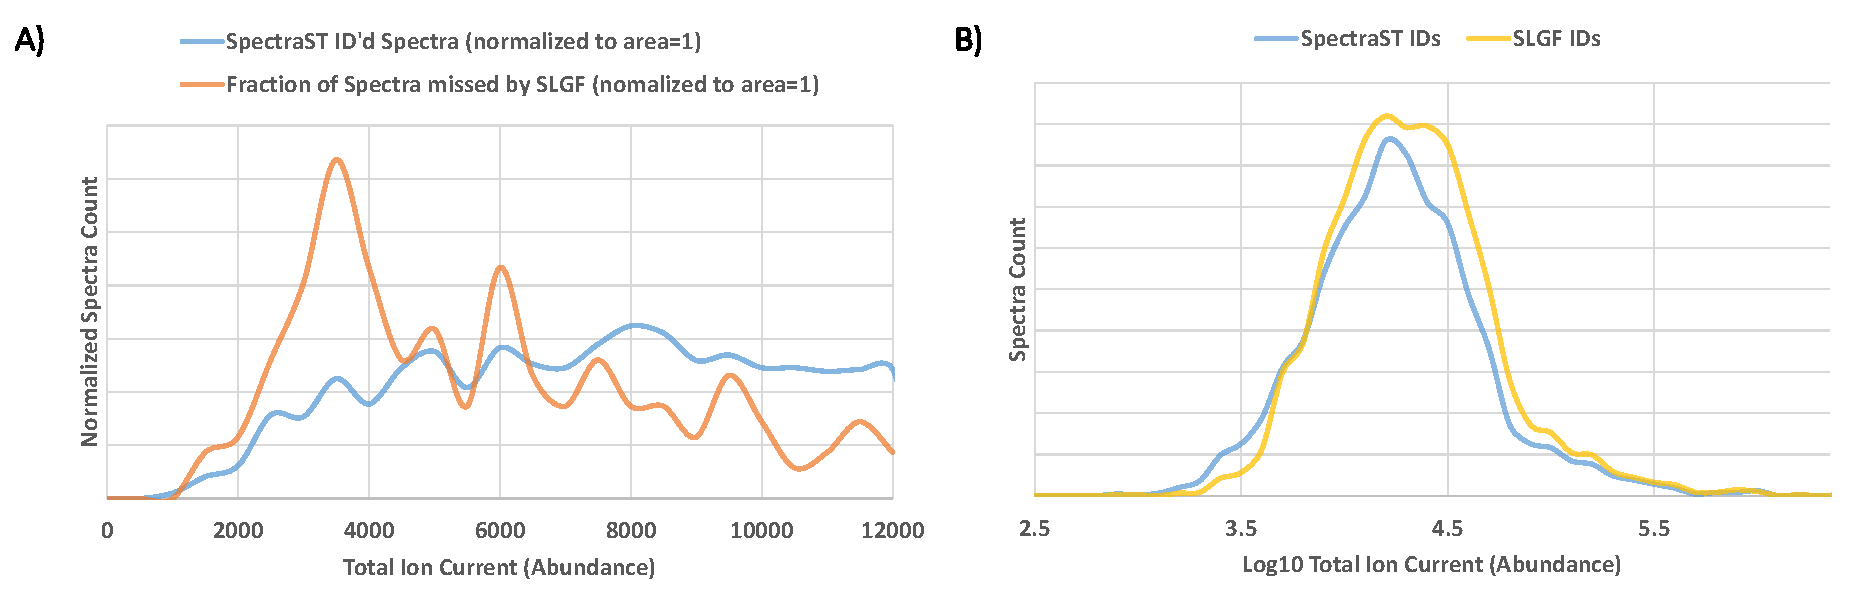
\includegraphics[scale=0.5]{Abundances2.pdf}
	\vspace{-0.1in}
  \caption{Distribution of peptide abundances for unidentified low abundance spectra
  %compared against distribution of abundances of low abundance training spectra, and a comparison in abundance distribution between identifications at 1\% FDR on the Training dataset.
  and spectra identified at 1\% FDR on the Training dataset. A) Low abundance spectra that were not identified by SLGF but were identified by SpectraST (in orange) on the Test dataset at 1\% FDR. In blue is the distribution of abundances for SpectraST identifications in the Training dataset and subsequently used to train SLGF. (B) Distribution of peptide abundances for IDs at 1\% FDR on the Test dataset, with SLGF shown in yellow and SpectraST in blue. SLGF is found to be more sensitive in regions of high abundance ($>12000$ ions) but loses some sensitivity in the very low abundance region. The loss of these identifications is caused in part by the low abundance ion variation model being trained on spectra mostly in the 5000-12000 ions range and thus not optimally modeling variation in spectra in the $<5000$ ions range.
  %, thus causing spike in missed low abundance identifications seen in (A).
  }
	\label{SearchAbundance}
\end{figure}

Missed identifications by SLGF on spectra from high abundance precursors separated into several categories as shown in Table~\ref{MissedSpectraTable}. Many examples of deamidation (a post translational modification that increases the mass of amino acids N or Q by 1 Da) were seen throughout our analysis for SpectraST is unable to distinguish between the two variants of the peptide because of the peak smoothing in SpectraST's spectrum preprocessing. However, we were able to distinguish these cases and {\em correctly} not identify them because deamidated versions of spectra were not present in the library. While identifying modified peptides from unmodified spectra is a worthy goal~\cite{bandeira07pnas}, we argue that such searches should \emph{explicitly} identify query spectra as modified variants of library spectra instead of just reporting them as the same unmodified peptide identification.

\begin{table}[!h]
  \centering
	\begin{tabular}{l*{1}{c}r}
	Reason              & Number of spectra  \\
	\hline
	Low Abundance Deamidation or 1 \ce{^{13}C} & 105 \\
	Low Abundance precursor m/z with $>2$ \ce{^{13}C}  &  36\\
	Low Abundance Other  &  193\\
	High Abundance  Deamidation or 1 \ce{^{13}C}           & 60   \\
	High Abundance precursor m/z with $>2$ \ce{^{13}C}        & 63  \\
	High Abundance Other  &  214\\
	\hline
	Total     & 671   \\
	\end{tabular}
  \caption{SpectraST identifications missed by SLGF at 1\% FDR. There were a total of 334 high abundance and 337 low abundance spectra that were missed by SLGF at 1\% FDR. While the numbers are comparable, the proportion of low abundance IDs missed was much higher as there were only $\sim 1400 $ low abundance spectra identified by SLGF at 1\% FDR. This higher percentage of missed low abundance spectra can be attributed to suboptimal SLGF models for very low abundance spectra as described in the text and in Figure~\ref{SearchAbundance}. }
	\label{MissedSpectraTable}
\end{table}

Additionally, 63 spectra contained a high number ($>2$) of \ce{^{13}C} isotope atoms. In these cases \ce{^{13}C} replaced the more common \ce{^{12}C} in the peptide, causing an increase in precursor mass because of the additional neutrons. The presence of these \ce{^{13}C} also affects the prefix and suffix ions in the MS/MS spectra as they skew a portion of the intensity of the b,y,b++,y++, etc. ions into peaks of 1 Da higher mass. This distorts the shape of the spectrum and exaggerates the variance in ion intensities of the query spectrum beyond what is expected by the SLGF distributions.

Of the remaining 214 other spectra that were not identified by SLGF at 1\% FDR, we manually examined a representative subset of these cases and determined that $\sim 30\%$ of spectra contained a mixture of two or more peptides. Another $\sim 23\%$ were matched to library spectra of questionable quality, exhibiting low signal to noise ratio and a high proportion of un-annotated peaks in the reference spectrum. While we have a low abundance ion variation model that accounts for low abundance {\em query} spectra matched to high quality library spectra, we could not account for lower quality library spectra since this information is not readily available. Several of these cases of lower quality library spectra were replaced in the subsequent release of the NIST yeast IT library indicating that NIST revisions also concluded that these library spectra were of lower quality. $\sim 28\%$ of the spectra were matched to high quality library spectra and exhibited high SSM cosine scores ($\sim 0.85$) but SLGF distributions were too strict (e.g., expected mean cosine was too high), which may indicate that we our average model of variation of ion intensities across all library spectra may not be the most appropriate for specific library peptides resulting in less reproducible spectra. % The remaining $19\%$ of the 214 spectra were attributed to a variety of causes, none of which seemed to constitute a trend.

In addition to comparing search performance on the {\em Yeast test dataset}, the {\em Hela S3 Test} dataset was searched against the NIST human ion trap spectral library using both $SLGF_{e}$ and SpectraST. Filtering to 1\% FDR (again determined by TDA), SLGF was able to identify 7433 MS/MS spectra compared to SpectraST's 6723 MS/MS spectra, yielding a 10.5\% increase in IDs. Note that since we calculated the SLGF theoretical distributions for the NIST human library using the ion variance models trained on the CPTAC {\em training dataset}, the amount of ion variation seemed to be understated compared to what we were seeing in the human data. To adjust for this higher variability in ion intensities, we shifted the SLGF theoretical distributions slightly lower. 


%Additionally, the {\em Study 8 LTQ} was searched against the NIST Yeast Spectral Library in the same fashion and parameters as {\em Test dataset}. The search performance of SLGF exhibited a similar pattern as the {\em Test dataset}, i.e. SLGF outperforms SpectraST on high abundance Spectra. At 1\% FDR, SLGF identified 12373 spectra versus SpectraST's 11402, representing an 8.5\% increase in IDs. Again mirroring the results from {\em Test dataset}, SLGF performed less optimally when identifying low abundance spectra. Given tis gain in identification rate of the high abundance spectra, it is clear that the ion variation model that was trained on data generated on different instruments from different labs, was suitable for the  {\em Study 8 LTQ} dataset for high abundance spectra. However, it is not safe to assume that our ion variation models are appropriate across different fragmentation modes (e.g. ETD, HCD) or across different vendors of instruments. Thus arises the need to create ion variation models for each of these classes of instruments. While we described our training set as consisting of millions of spectra, such a large quantity of spectra is not necessary. Tens of thousands of identified replicate spectra are sufficient to calculate the ion variation model and for most instruments this quantity of spectra can be easily acquired. 



\subsection*{Conclusion}

Having been repeatedly found~\cite{lam07,yen11,lam10methods,dasari12} that spectral library searching performs consistently better than database search of the same peptide identification search space in high-throughput proteomics, there is now renewed interest in establishing statistical methods to further assess the quality of Spectrum-Spectrum Matches (SSMs) and increase the total number of reported SSM-based identifications. Here we propose a new Spectral Library Generating Function (SLGF) approach to assessing the significance of SSMs, show how to rigorously calculate SLGF distributions for any spectrum from any type of molecule and demonstrate that SLGF-based peptide spectral library searching identifies significantly more spectra than state-of-the-art alternative search tools. In difference from database search (and other fields) where statistical significance is estimated by calculating the p-value of observing a high match score when matching a random sequence, we circumvent the open problem of defining realistic `random' MS/MS spectra by instead calculating the p-value of observing a low match score when matching a true (replicate) spectrum to a known reference spectrum. To achieve this goal, we explicitly model instrument variation in measurement of MS/MS peak intensities and show how these can be used to derive theoretical distributions of SSM cosines between replicate and reference library spectra.

%We propose and evaluate the performance of a new Spectral Library Generating Function (SLGF) approach to estimate the significance of Spectrum-Spectrum Matches (SSMs) based on a different null hypothesis than has traditionally been considered. Instead of modeling the distributions of `random' SSMs to assign p-values to true SSMs
%
%query spectra as random spectra or as if arising from random peptide sequences, we model query spectra as replicates of library spectra.

%It has been shown that this approach, SLGF, improved peptide identification rates in proteomics spectral library search, in comparing against the state of the art SpectraST at fixed FDR. Our analysis further showed that SLGF probabilities assign significance to cosine scores such that additional corrections to the score (e.g. $DotBias$ and $DeltaD$) are no longer necessary.

Despite marked gains over Pepitome~\cite{dasari12} and SpectraST~\cite{lam07}, our results suggest that 3 levels of precursor intensity models ($<5000$ ions, $5000-12000$ ions, $>12000$ ions) may be better suited to model peak intensity variations across the range of precursor abundances in our sample and could thus further improve SLGF's performance. In addition, while our models take into consideration the precursor abundance for query spectra, it would also be informative to know the precursor abundance of library spectra since fragmentation patterns in these are also very dependent on precursor abundance. Further studies will be able to determine the effect of both of these factors through the use of larger training and reference datasets.

Currently, one limitation of the SLGF model is that it only takes into account peak intensity variation and peak deletion in query spectra, not insertions. This feature would aid in the detection of spurious noise peaks and further filter out random matches, and is a planned feature for SLGF. There are however certain complications, as the probably of an insertion is highly dependent upon the intensity of the inserted peak. Thus, further investigation is nessary on determining the appropriate method of modeling peak insertions. 

Even though we did not explicitly aim to identify mixture spectra (and did not evaluate it), we note that the proposed SLGF approach is based on matching reference library spectra to {\em subsets} of peaks in query spectra (i.e., normalized projections) and thus appears to be well suited to determining \emph{containment} of compounds in mixture spectra. While a detailed assessment of SLGF's performance on mixture spectra would require a more comprehensive evaluation~\cite{wang10}, our preliminary results illustrated in Figure~\ref{SLGFSearchROCVenn}A show that SLGF's performance was essentially indistinguishable from that of $SLGF_e$ and thus strongly suggests that SLGF should be suitable for identification of peptides in mixture spectra.


{\bf Acknowledgements. }
The authors would like to thank David Tabb and Nathan Edwards for providing the CPTAC data used in our Training and Test datasets. This work was supported by the National Institutes of Health grant 3-P41-GM103484 from the National Institute of General Medical Sciences.


\newpage

\bibliographystyle{plain}	% (uses file "plain.bst")
\bibliography{../../bibtex/msms,../../bibtex/bandeiraLab}		% expects file "myrefs.bib"

\end{document} 